
% Copyright (c) 2015 - 2019 Mario Mlačak, mmlacak@gmail.com
% Licensed and published as Public Domain work.

% Discovery chapter ===================================================
\chapter*{Discovery}
\addcontentsline{toc}{chapter}{Discovery}

\begin{flushright}
\parbox{0.8\textwidth}{
\emph{I don’t believe in God but I’m very interested in her. \\
\hspace*{\fill}{\textperiodcentered \textperiodcentered \textperiodcentered \hspace*{0.2em} Arthur C. Clarke} } }
\end{flushright}

\noindent
Discovery is chess variant which is played on 24 x 24 board, with
light (pastel!) yellow and gray fields and darker gray and dark teal
pieces. Star colors are bright orange and dark violet. In algebraic
notation, columns are enumerated from 'a' to 'x', and rows are
enumerated from '1' to '24'. A new piece is introduced, Monolith.

\clearpage % ..........................................................
% Monolith ************************************************************

\section*{Monolith}
\addcontentsline{toc}{section}{Monolith}

\noindent
\begin{wrapfigure}[10]{l}{0.4\textwidth}
\centering
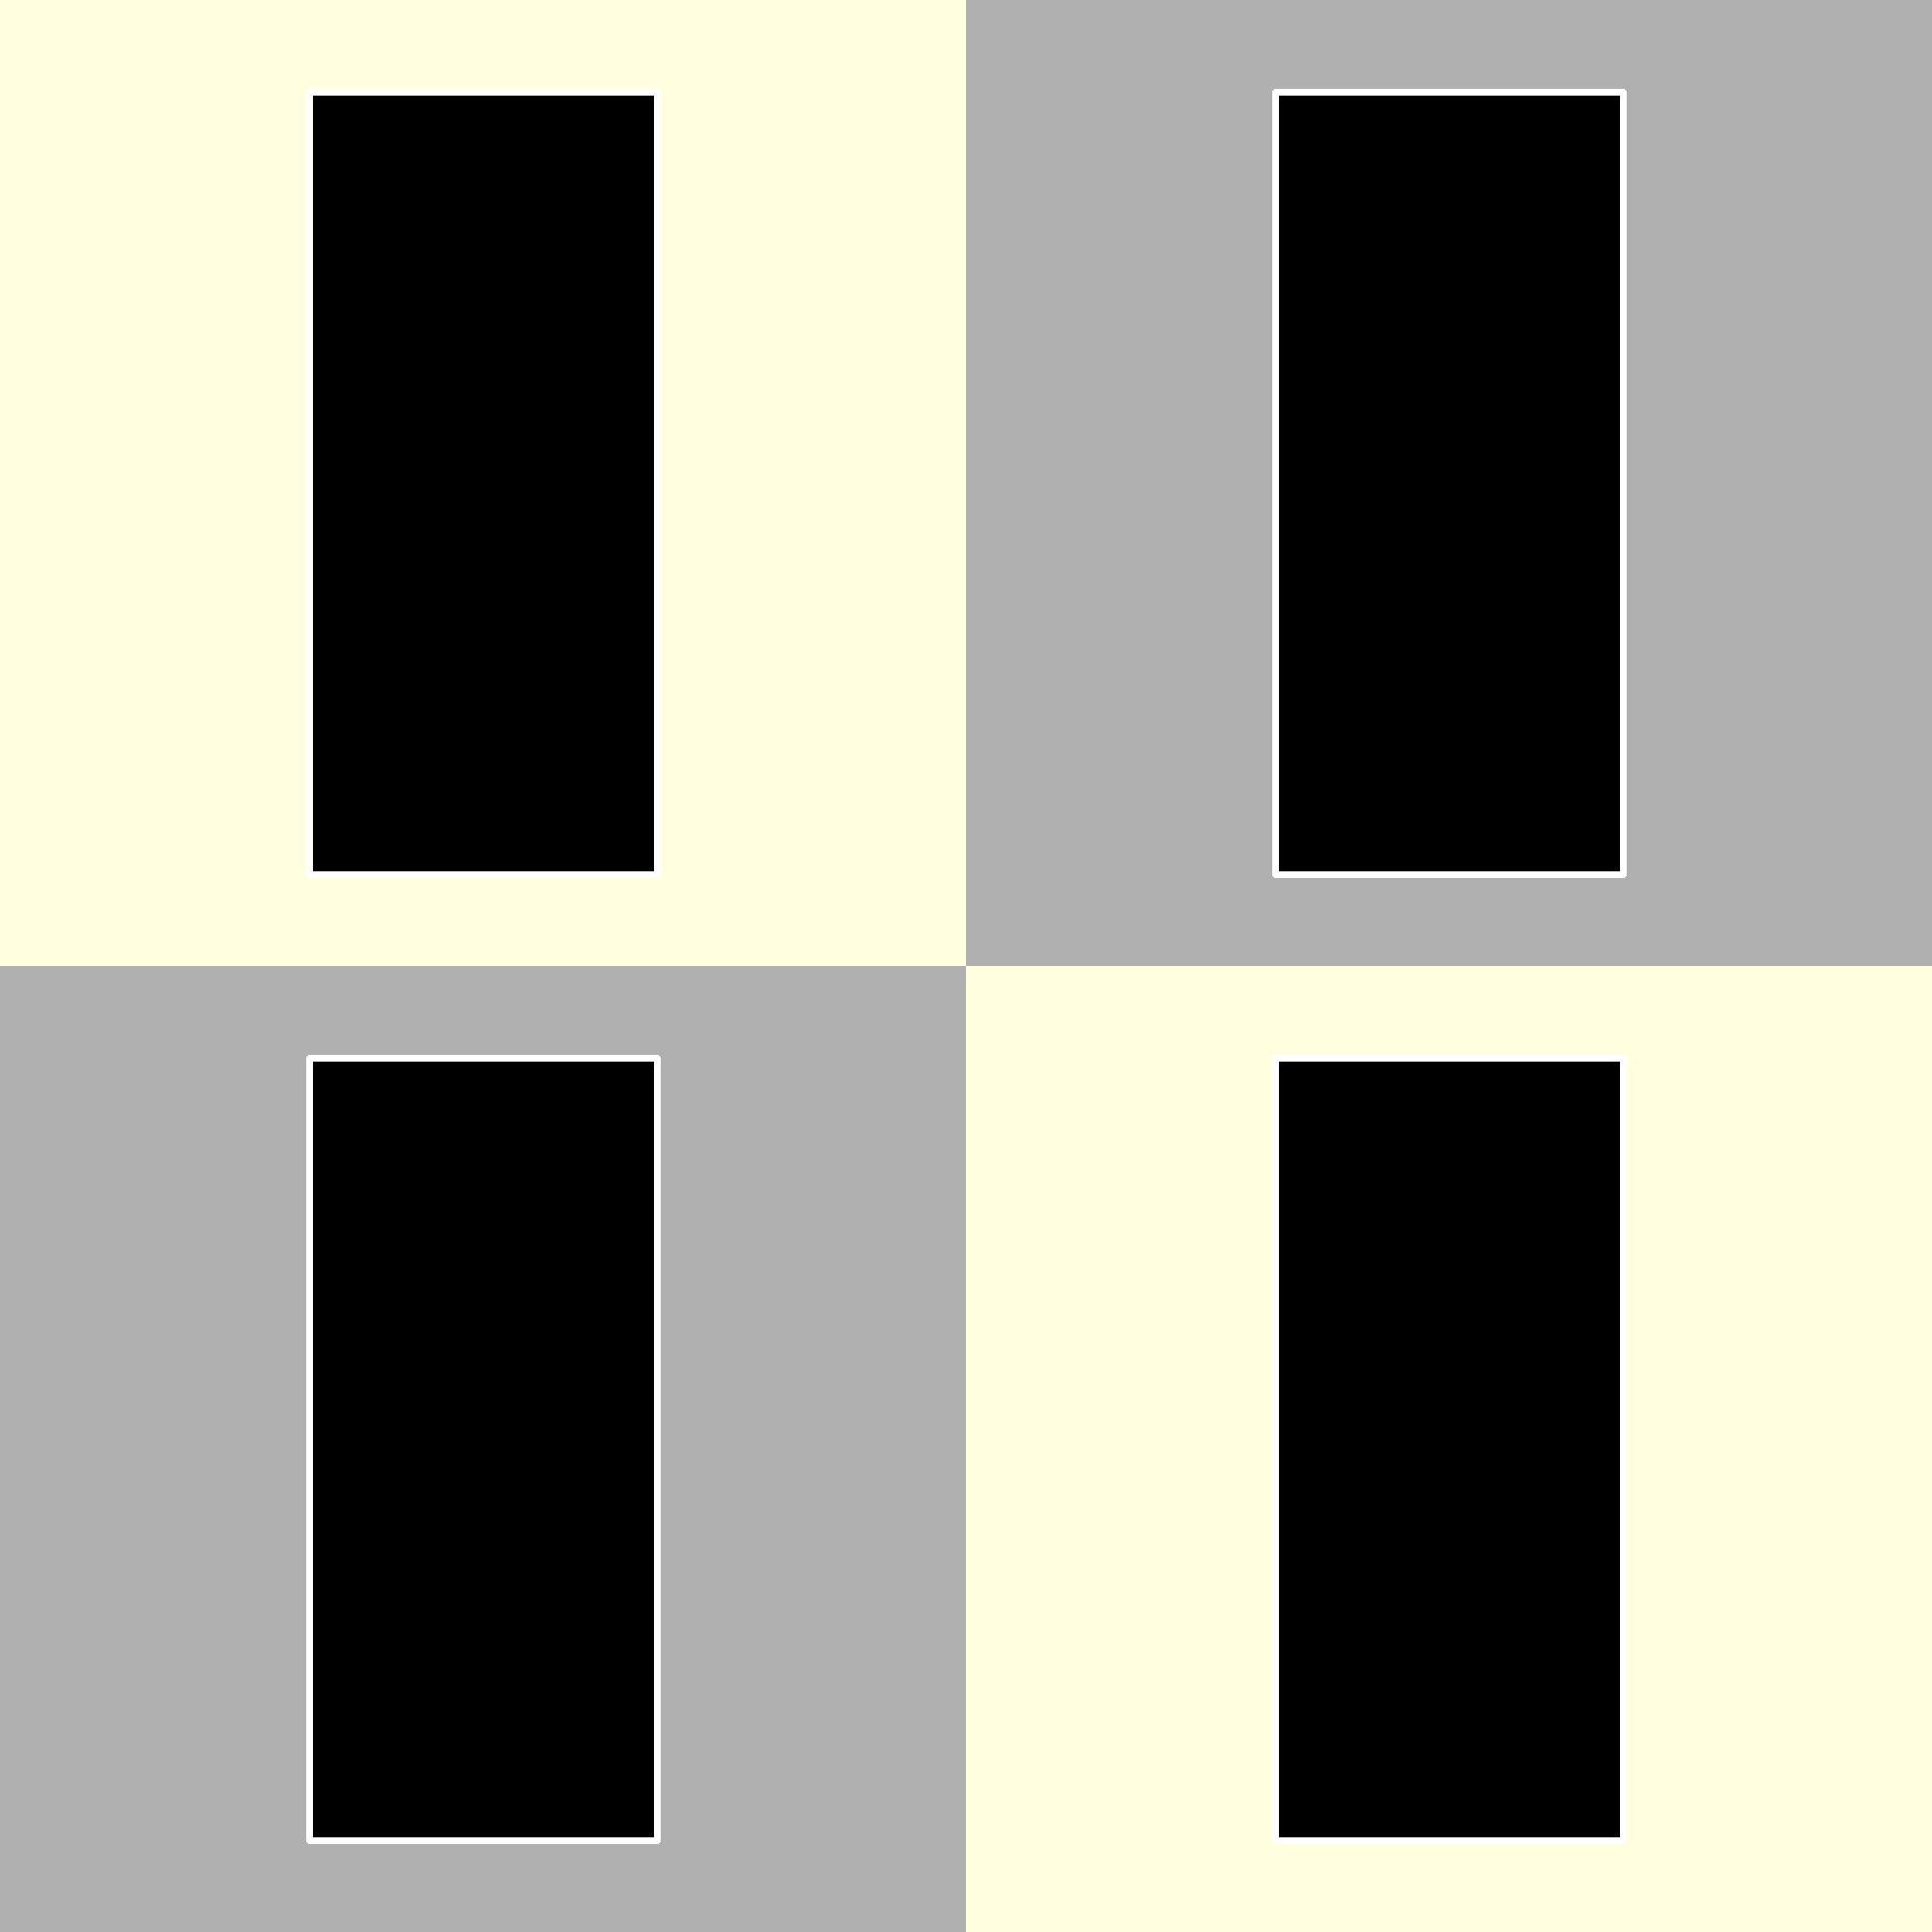
\includegraphics[width=0.4\textwidth, keepaspectratio=true]{pieces/15_monolith.png}
\caption{Monolith}
\label{fig:15_monolith}
\end{wrapfigure}
Monolith does not belong to any player, but can be moved by both of them.

Monolith is a teleportation device, much like moveable Star. Player can use
any Star or the other Monolith as a destination.

Monolith cannot be captured, converted, nor activated.
Pawn cannot be promoted to Monolith.

[?] Syzygy ... [?]

[?] Hybrid ... Wave activates Monolith, others are teleported by Monolith [?]

In algebraic notation, symbol for Monolith is 'M'.

\vspace*{0.05\textheight}
\noindent
\begin{wrapfigure}[2]{l}{0.4\textwidth}
\centering
\includegraphics[width=0.4\textwidth, keepaspectratio=true]{pieces/bishop/20_discovery.png}
\caption{Bishop}
\label{fig:bishop/20_discovery}
\end{wrapfigure}
Piece colors in this variant are presented on the left.

\clearpage % ..........................................................

% \vspace*{0.25\textheight}
\noindent
\begin{wrapfigure}[2]{l}{0.4\textwidth}
\centering
\includegraphics[width=0.4\textwidth, keepaspectratio=true]{pieces/star/20_discovery.png}
\caption{Star}
\label{fig:star/20_discovery}
\end{wrapfigure}
Star colors in this variant are presented on the left.

% \clearpage % ..........................................................
% Movement ------------------------------------------------------------

\vspace*{0.35\textheight}

\subsection*{Movement}
\addcontentsline{toc}{subsection}{Movement}

% \vspace*{0.05\textheight}
\noindent
\begin{wrapfigure}{l}{0.35\textwidth} % [11]
\centering
\includegraphics[width=0.291666667\textwidth, keepaspectratio=true]{examples/20_d/scn_d_01_monolith_diagonals.png}
\caption{Monolith diagonals}
\label{fig:scn_d_01_monolith_diagonals}
\end{wrapfigure}
...

\clearpage % ..........................................................

\noindent
\begin{figure}[!h]
% \begin{figure}[!t]
\includegraphics[width=1.0\textwidth, keepaspectratio=true]{examples/20_d/scn_d_02_monolith_step_2.png}
\caption{Monolith step 2}
\label{fig:scn_d_02_monolith_step_2}
% \centering
\end{figure}

...

\clearpage % ..........................................................

\huge{TODO :: Shaman's trance-journey interaction}
\normalsize{}
...

% ------------------------------------------------------------ Movement
% ************************************************************ Monolith
\clearpage % ..........................................................

\section*{Promotion}
\addcontentsline{toc}{section}{Promotion}

Promotion is non enforced, delayed variety, i.e. it's the same as in
\hyperref[sec:Age of Aquarius/Promotion]{previous chess variant}, Age of Aquarius.

Promotion in this variant is polygamous, more than one Queen in the same color
can be present on chessboard at any given time.

Again, Pawn cannot be promoted to Monolith.

\clearpage % ..........................................................

\section*{En passant}
\addcontentsline{toc}{section}{En passant}

\noindent
\begin{wrapfigure}{l}{0.4\textwidth}
\centering

\includegraphics[width=0.125\textwidth, keepaspectratio=true]{en_passants/20_discovery_en_passant.png}
\caption{En passant}
\label{fig:20_discovery_en_passant}
\end{wrapfigure}
Rush and en passant are identical to those in Classic Chess, only difference
is that Pawn can now move longer on initial turn, up to 10 fields in this
variant.

\clearpage % ..........................................................

\section*{Castling}
\addcontentsline{toc}{section}{Castling}

Castling is the same as in Classical Chess, only difference is that King can move between 2 and 9 fields across.
All other constraints from Classical Chess still applies.

\noindent
\begin{figure}[!h]
% \begin{figure}[!t]
\includegraphics[width=1.0\textwidth, keepaspectratio=true]{castlings/20_d/discovery_castling.png}
\caption{Castling}
\label{fig:discovery_castling}
% \centering
\end{figure}

In example above, all valid King's castling moves are numbered.

\noindent
\begin{figure}[!h]
% \begin{figure}[!t]
\includegraphics[width=1.0\textwidth, keepaspectratio=true]{castlings/20_d/discovery_castling_left_07.png}
\caption{Castling long left}
\label{fig:discovery_castling_left_07}
% \centering
\end{figure}

In this example King was castling long to the left. Initial King's position is marked with "K".
After castling is finished, left Rook ends up at field immediately right to the King.

\clearpage % ..........................................................

\section*{Initial setup}
\addcontentsline{toc}{section}{Initial setup}

Compared to initial setup of Conquest of Tlalocan, just 2 Monoliths are placed in to the open,
symetrically, on both sides of chessboard. This can be seen in the image below:

\noindent
% \begin{figure}[t]
\begin{figure}[h]
\includegraphics[width=1.0\textwidth, keepaspectratio=true]{boards/20_discovery.png}
\caption{Discovery board}
\label{fig:20_discovery}
% \centering
\end{figure}

\clearpage % ..........................................................
% =================================================== Discovery chapter
